\documentclass[9pt]{beamer}
\usetheme{CambridgeUS}
\usepackage{xcolor}
\usepackage{geometry}
\usepackage{array}
\usepackage{comment}

\AtBeginSection[]
{
  \begin{frame}
    \frametitle{Table of Contents}
    \tableofcontents[currentsection]
  \end{frame}
}

\setbeamertemplate{footline}
{
  \leavevmode%
  \hbox{%
    \begin{beamercolorbox}[wd=.333333\paperwidth,ht=2.25ex,dp=1ex,center]{author in head/foot}%
      \usebeamerfont{author in head/foot}\insertshortauthor
    \end{beamercolorbox}%
    \begin{beamercolorbox}[wd=.333333\paperwidth,ht=2.25ex,dp=1ex,center]{title in head/foot}%
      \usebeamerfont{title in head/foot}\insertshortsubtitle
    \end{beamercolorbox}%
    \begin{beamercolorbox}[wd=.333333\paperwidth,ht=2.25ex,dp=1ex,right]{date in head/foot}%
      \usebeamerfont{date in head/foot}\insertshortdate{}\hspace*{2em}
      \usebeamertemplate{page number in head/foot}\hspace*{2ex}
    \end{beamercolorbox}
  }%
  \vskip0pt%
}

\title{Principles of Economics}
\subtitle{Discussion Session 5: Costs and the Supply Curve}
\author{Joe Wilske}
\institute{Boston College}
\date{\today}

\begin{document}

\frame{\titlepage}

\begin{frame}{Types of Costs}

Imagine you own a restaurant...
\vspace{5pt}
    \begin{enumerate}
        \item \textbf{Fixed Costs:} Costs that must be paid whether the restaurant is operating or not.
        \begin{itemize}
            \item Rent, equipment leases, alcohol license renewal fees, ...
        \end{itemize}
        \vspace{5pt}
        \item \textbf{Variable Costs:} Costs that are only paid if the restaurant is operating.
        \begin{itemize}
            \item Labor, food supplies, electricity, ...
        \end{itemize}
        \vspace{5pt}
        \item \textbf{Total Cost:} The sum of fixed and variable costs. 
        \begin{itemize}
            \item $TC = FC + VC$    
        \end{itemize}
        \vspace{5pt}
        \item \textbf{Marginal Cost:}  The cost of the \textit{last unit produced}.
        \begin{itemize}
            \item If you produce $Q$ units, then\\
            \vspace{2pt}
            $MC_Q = VC_Q - VC_{Q-1}, \:$ or equivalently\\
            \vspace{2pt}
            $MC_Q = TC_Q - TC_{Q-1} = FC + VC_Q - (FC + VC_{Q-1}) = VC_Q - VC_{Q-1}$
        \end{itemize}
        \vspace{5pt}
        \item \textbf{Average Costs:} Just divide by the quantity produced.
        \begin{itemize}
            \item $AFC = FC/Q, \quad AVC = VC/Q, \quad ATC = TC/Q$
        \end{itemize}
    \end{enumerate}
\end{frame}


\begin{frame}{Exercise 1: Types of Costs}
    Fill in the following table: 
    \begin{table}[]
    \centering
    \begin{tabular}{ccccccc}
    \hline
    Q & VC  & TC  & AFC   & AVC & ATC   & MC  \\
    \hline
    0 &     & 50  & N/A   & N/A & N/A   & N/A  \\
    1 & 10  &     &       & 10  & 60    & 10  \\
    2 & 30  & 80  &       &     &       &   \\
    3 &     &     & 16.67 & 20  & 36.67 & 30  \\
    4 & 100 & 150 & 12.50 &     & 37.50 &   \\
    5 & 150 &     &       & 30  &       &   \\
    6 & 210 & 260 & 8.33  & 35  & 43.33 & 60  \\
    \hline
    \end{tabular}
\end{table}
\end{frame}

\begin{frame}{Exercise 1: Different Types of Costs}
    Solution: 
    \begin{table}[]
    \centering
    \begin{tabular}{ccccccc}
    \hline
    Q & VC  & TC  & AFC   & AVC & ATC   & MC  \\
    \hline
    0 & 0   & 50  & N/A   & N/A & N/A   & N/A  \\
    1 & 10  & 60  & 50    & 10  & 60    & 10  \\
    2 & 30  & 80  &  25   & 15  &  40   & 20 \\
    3 & 60  & 110 & 16.67 & 20  & 36.67 & 30  \\
    4 & 100 & 150 & 12.50 & 25  & 37.50 & 40 \\
    5 & 150 & 200 &   10  & 30  &   40  & 50 \\
    6 & 210 & 260 & 8.33  & 35  & 43.33 & 60  \\
    \hline
    \end{tabular}
\end{table}
\end{frame}

\begin{frame}{Cost Curves}
\begin{columns}[c]
    \begin{column}{0.5\textwidth}
        \begin{itemize}
            \item<1-> \textbf{Decreasing returns to scale:}\\
            The amount of input required to produce one more unit of output increases with quantity of output.\\
            $\implies$ MC is upward-sloping.
            \vspace{5pt}
            \item<2-> AVC decreases when greater than MC and increases when less than MC.\\
            $\implies$ MC crosses AVC at the minimum.
            \vspace{5pt}
            \item<3-> ATC adds average fixed cost to AVC\\
            $\implies$ Behaves in the same way as AVC.
        \end{itemize}
    \end{column}
    \begin{column}{0.5\textwidth}
        \only<1>{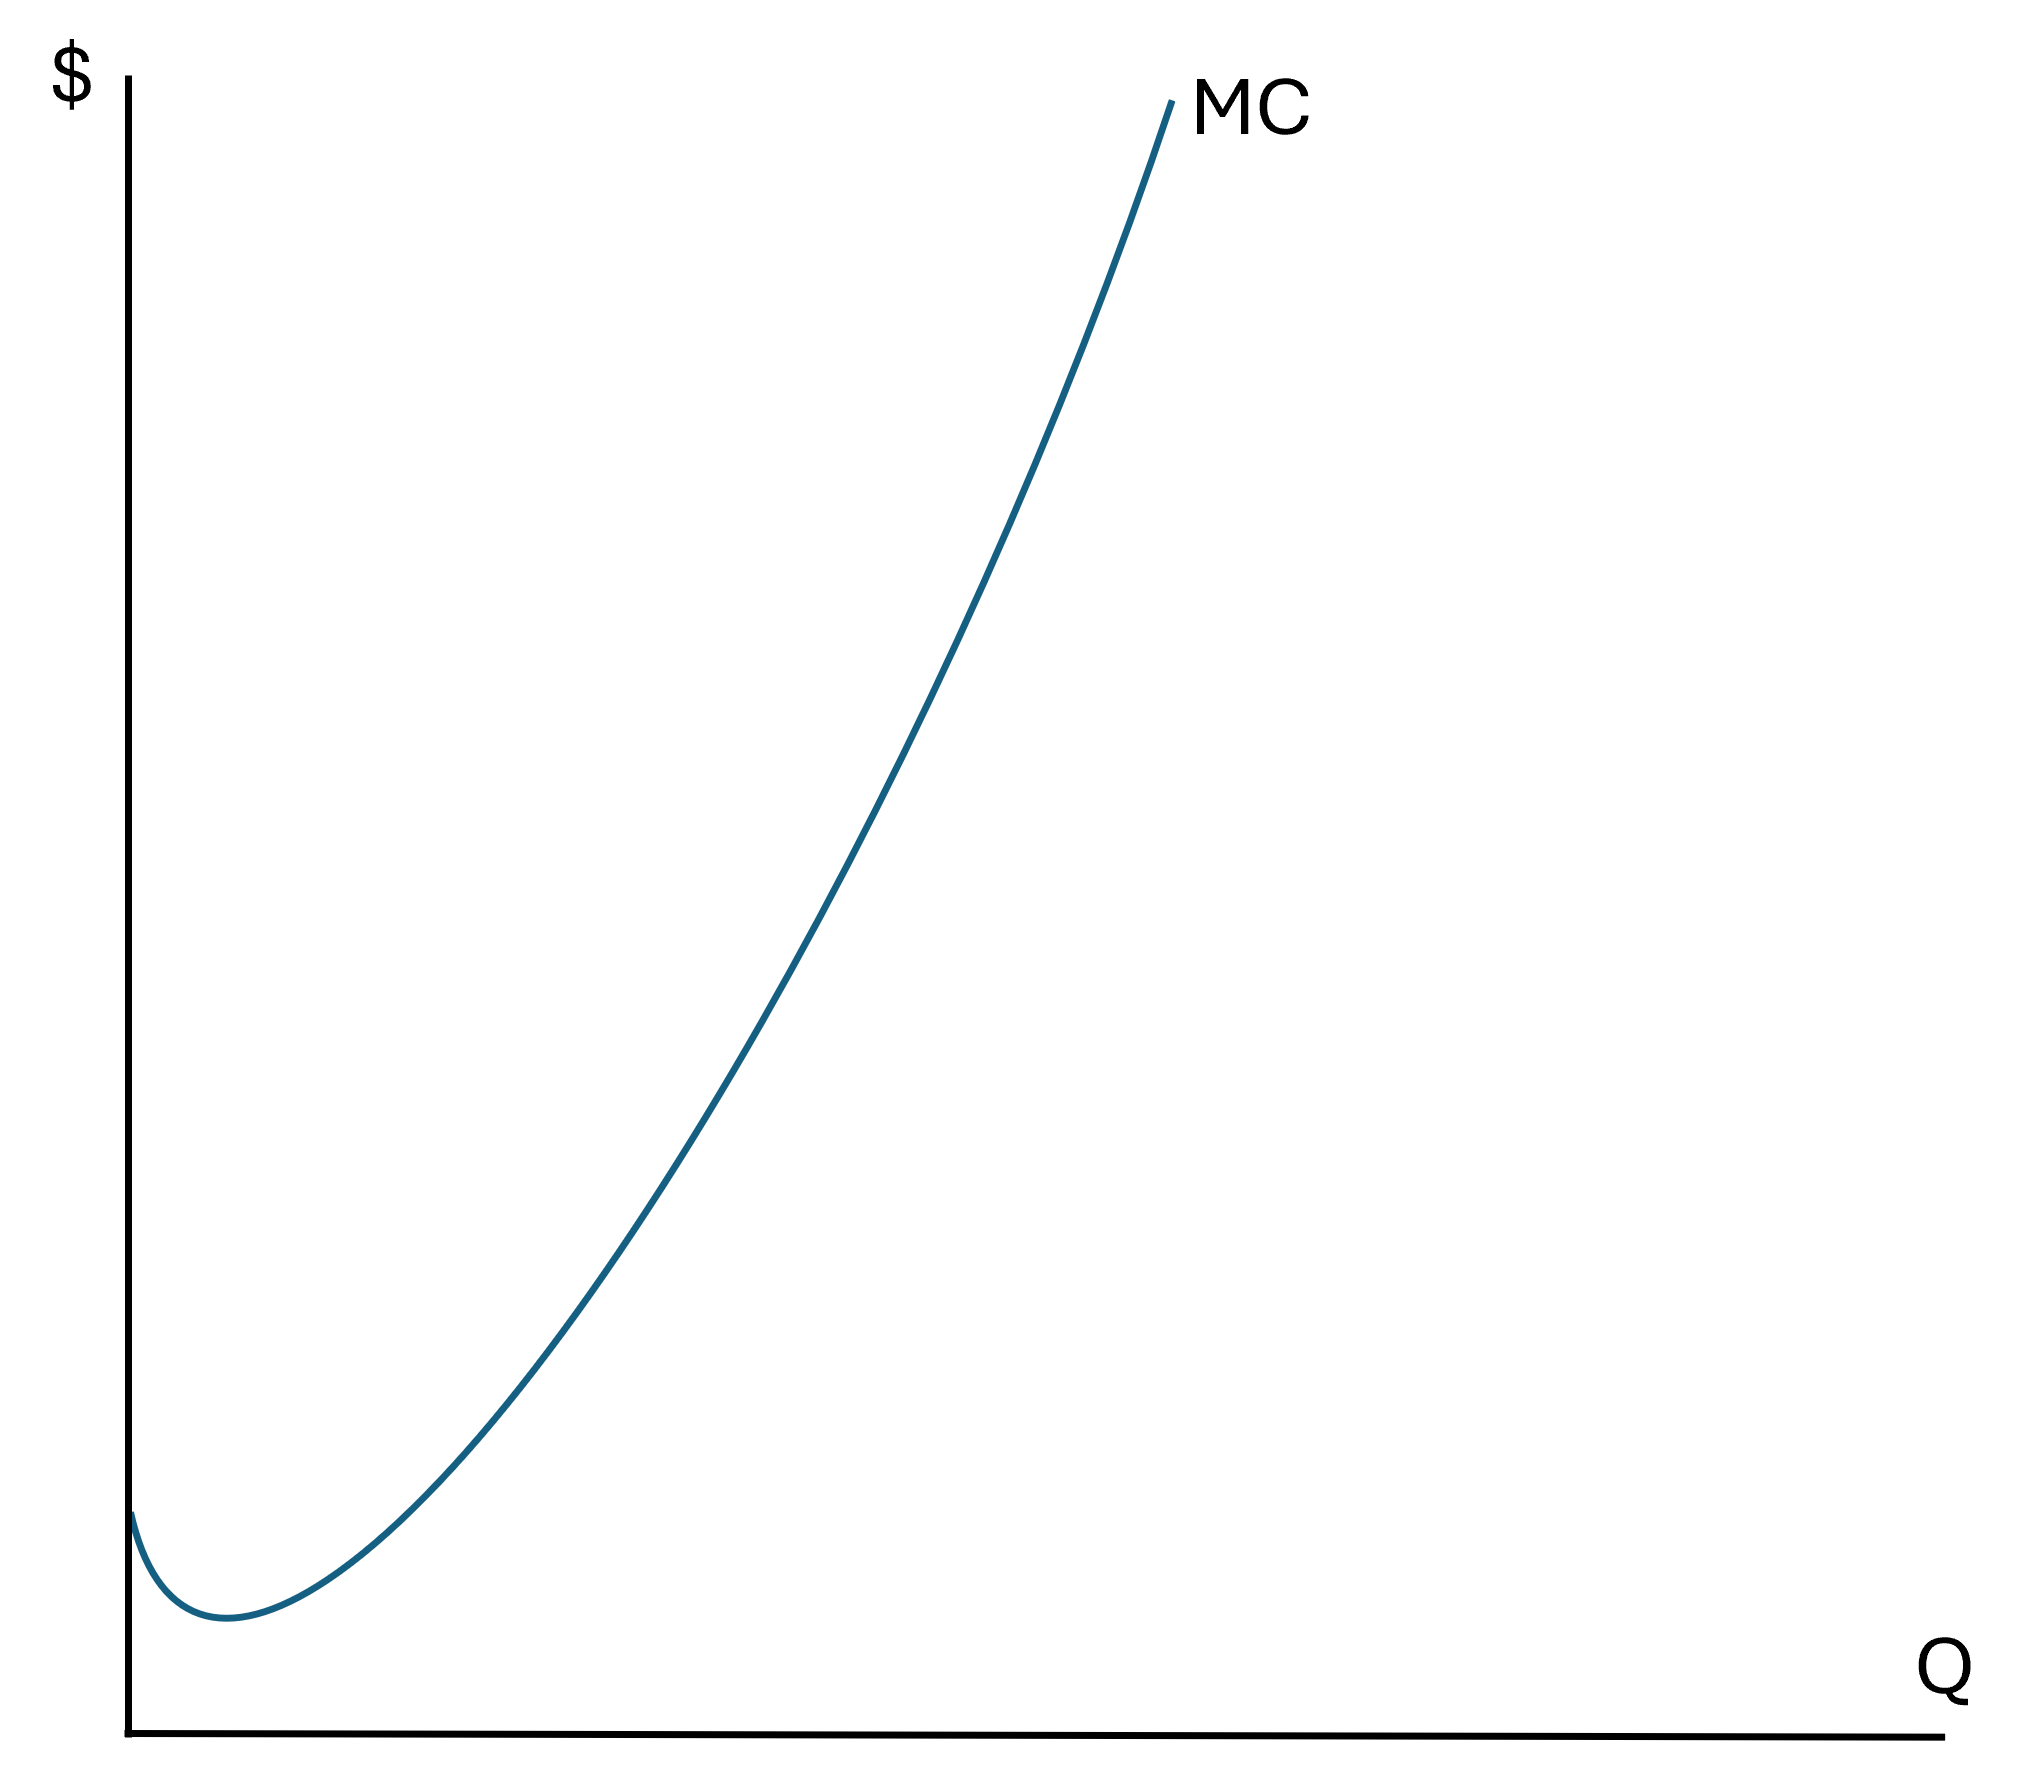
\includegraphics[width=\linewidth]{MC.png}}
        \only<2>{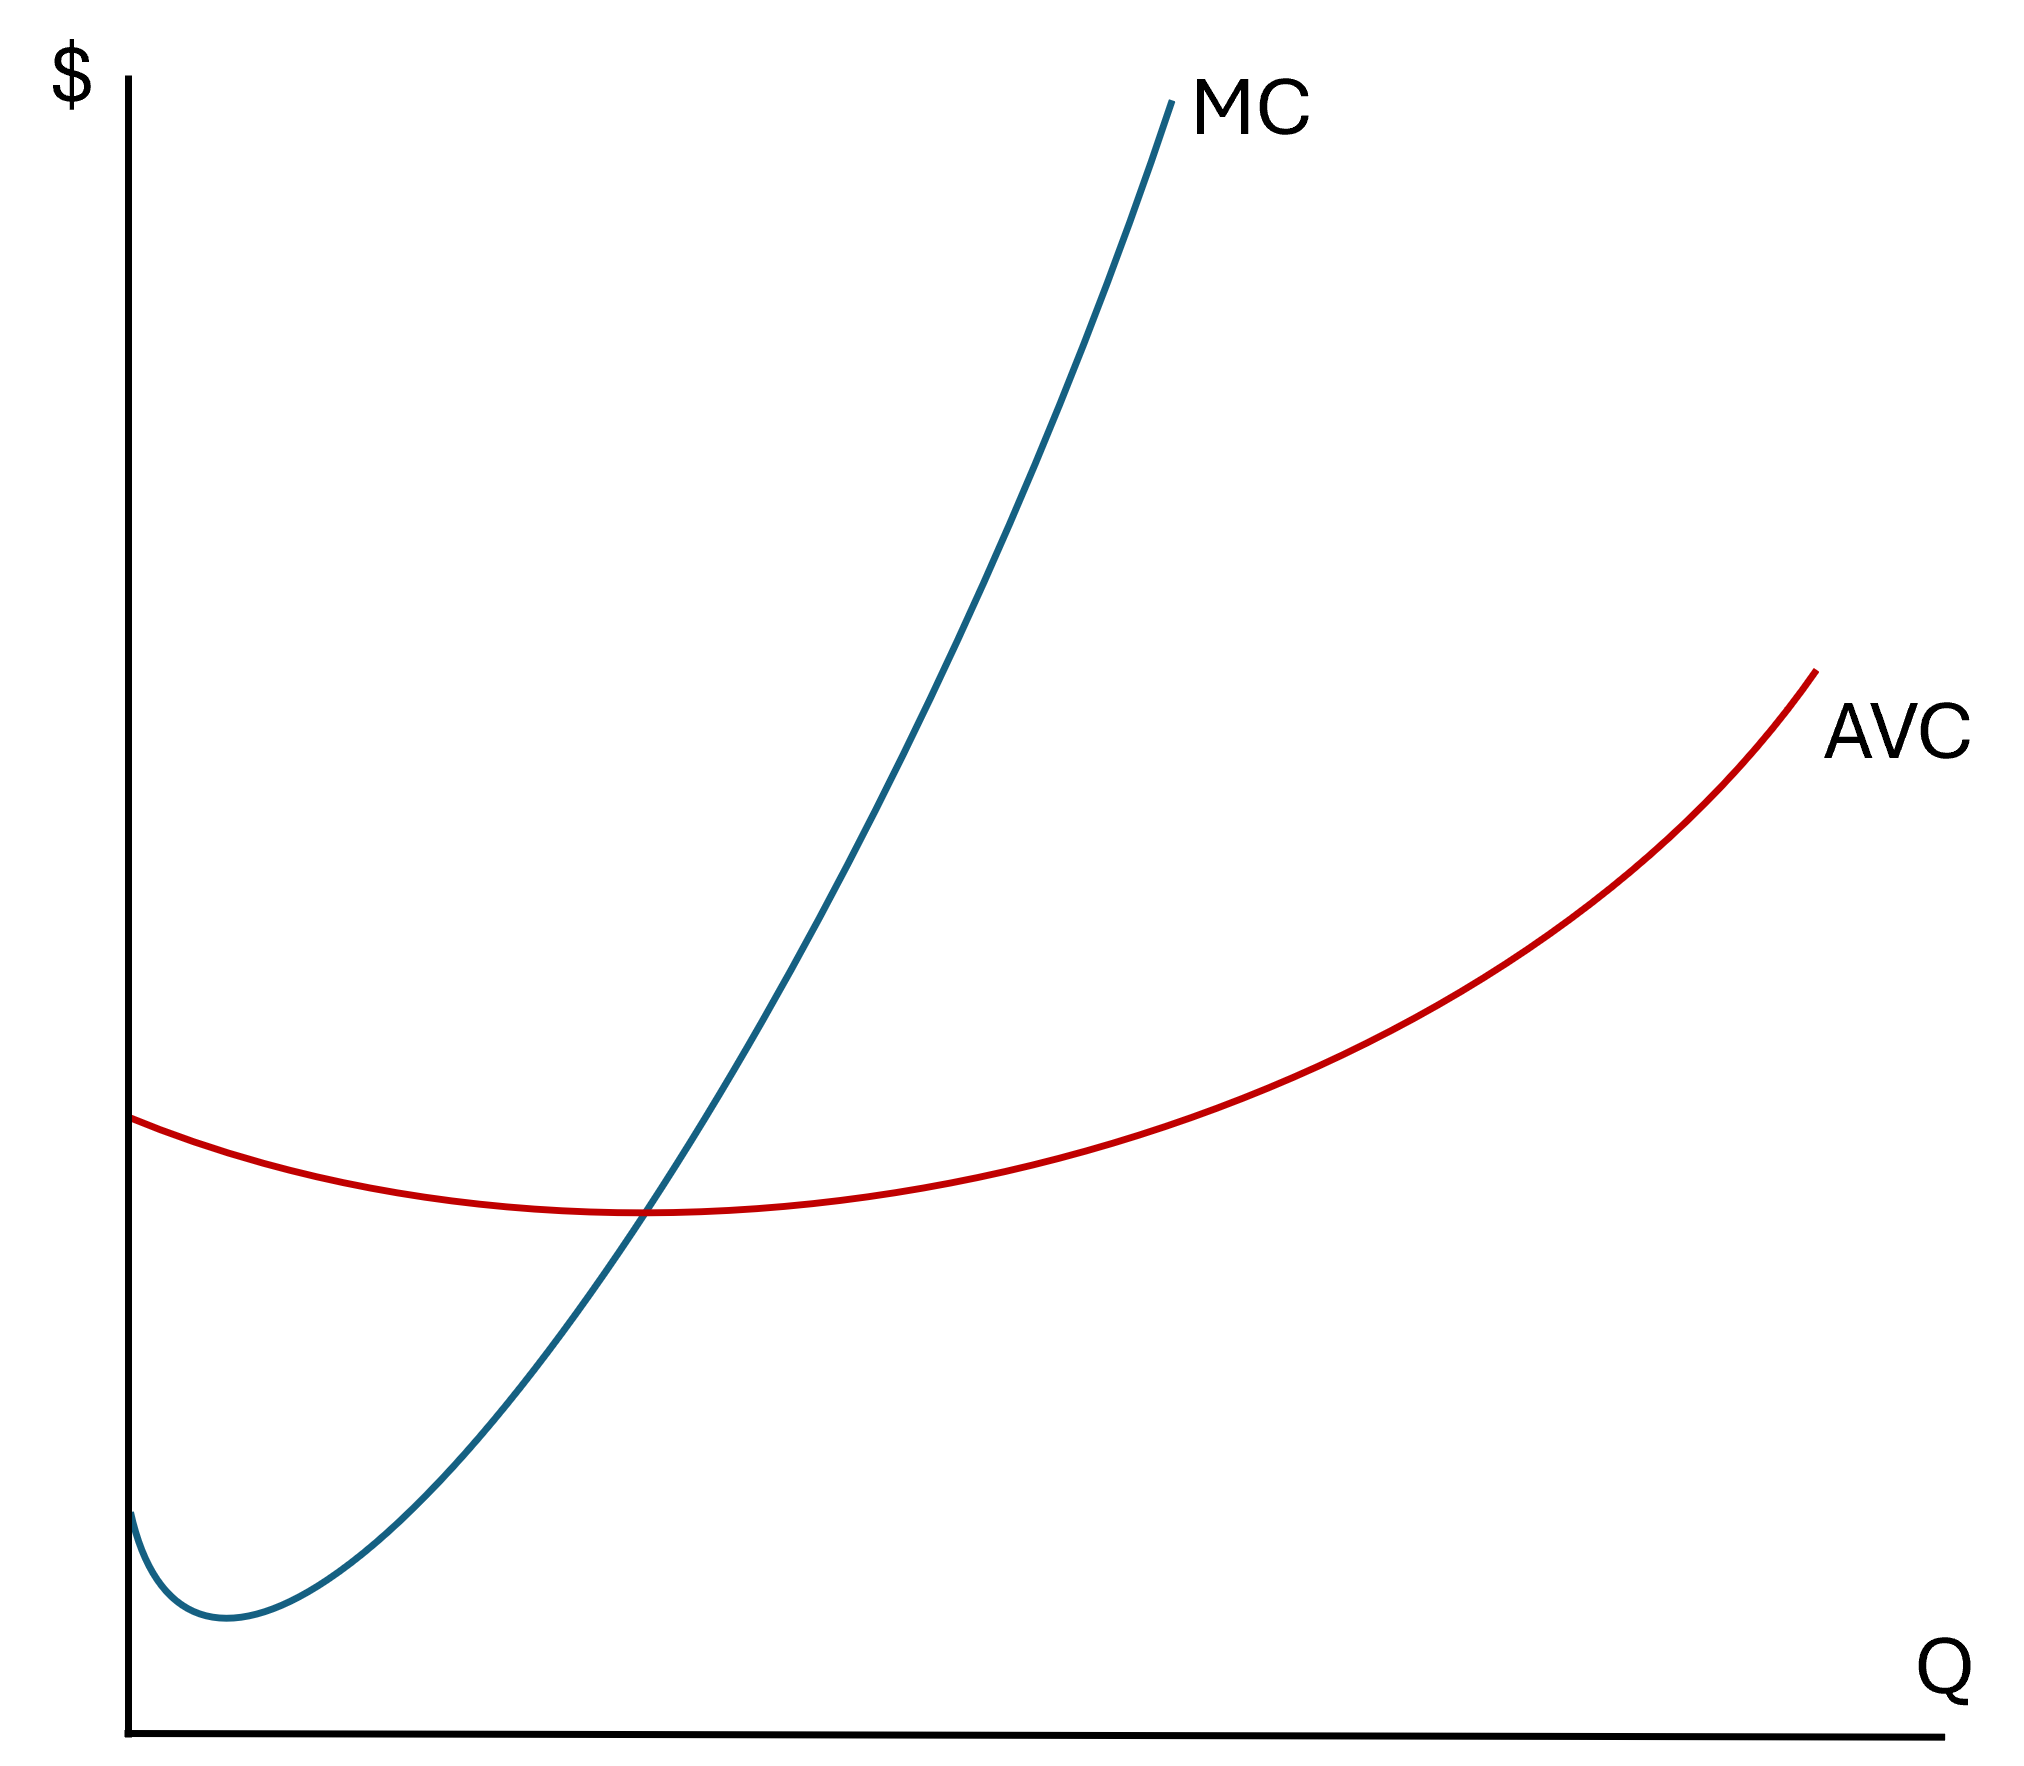
\includegraphics[width=\linewidth]{AVC.png}}
        \only<3>{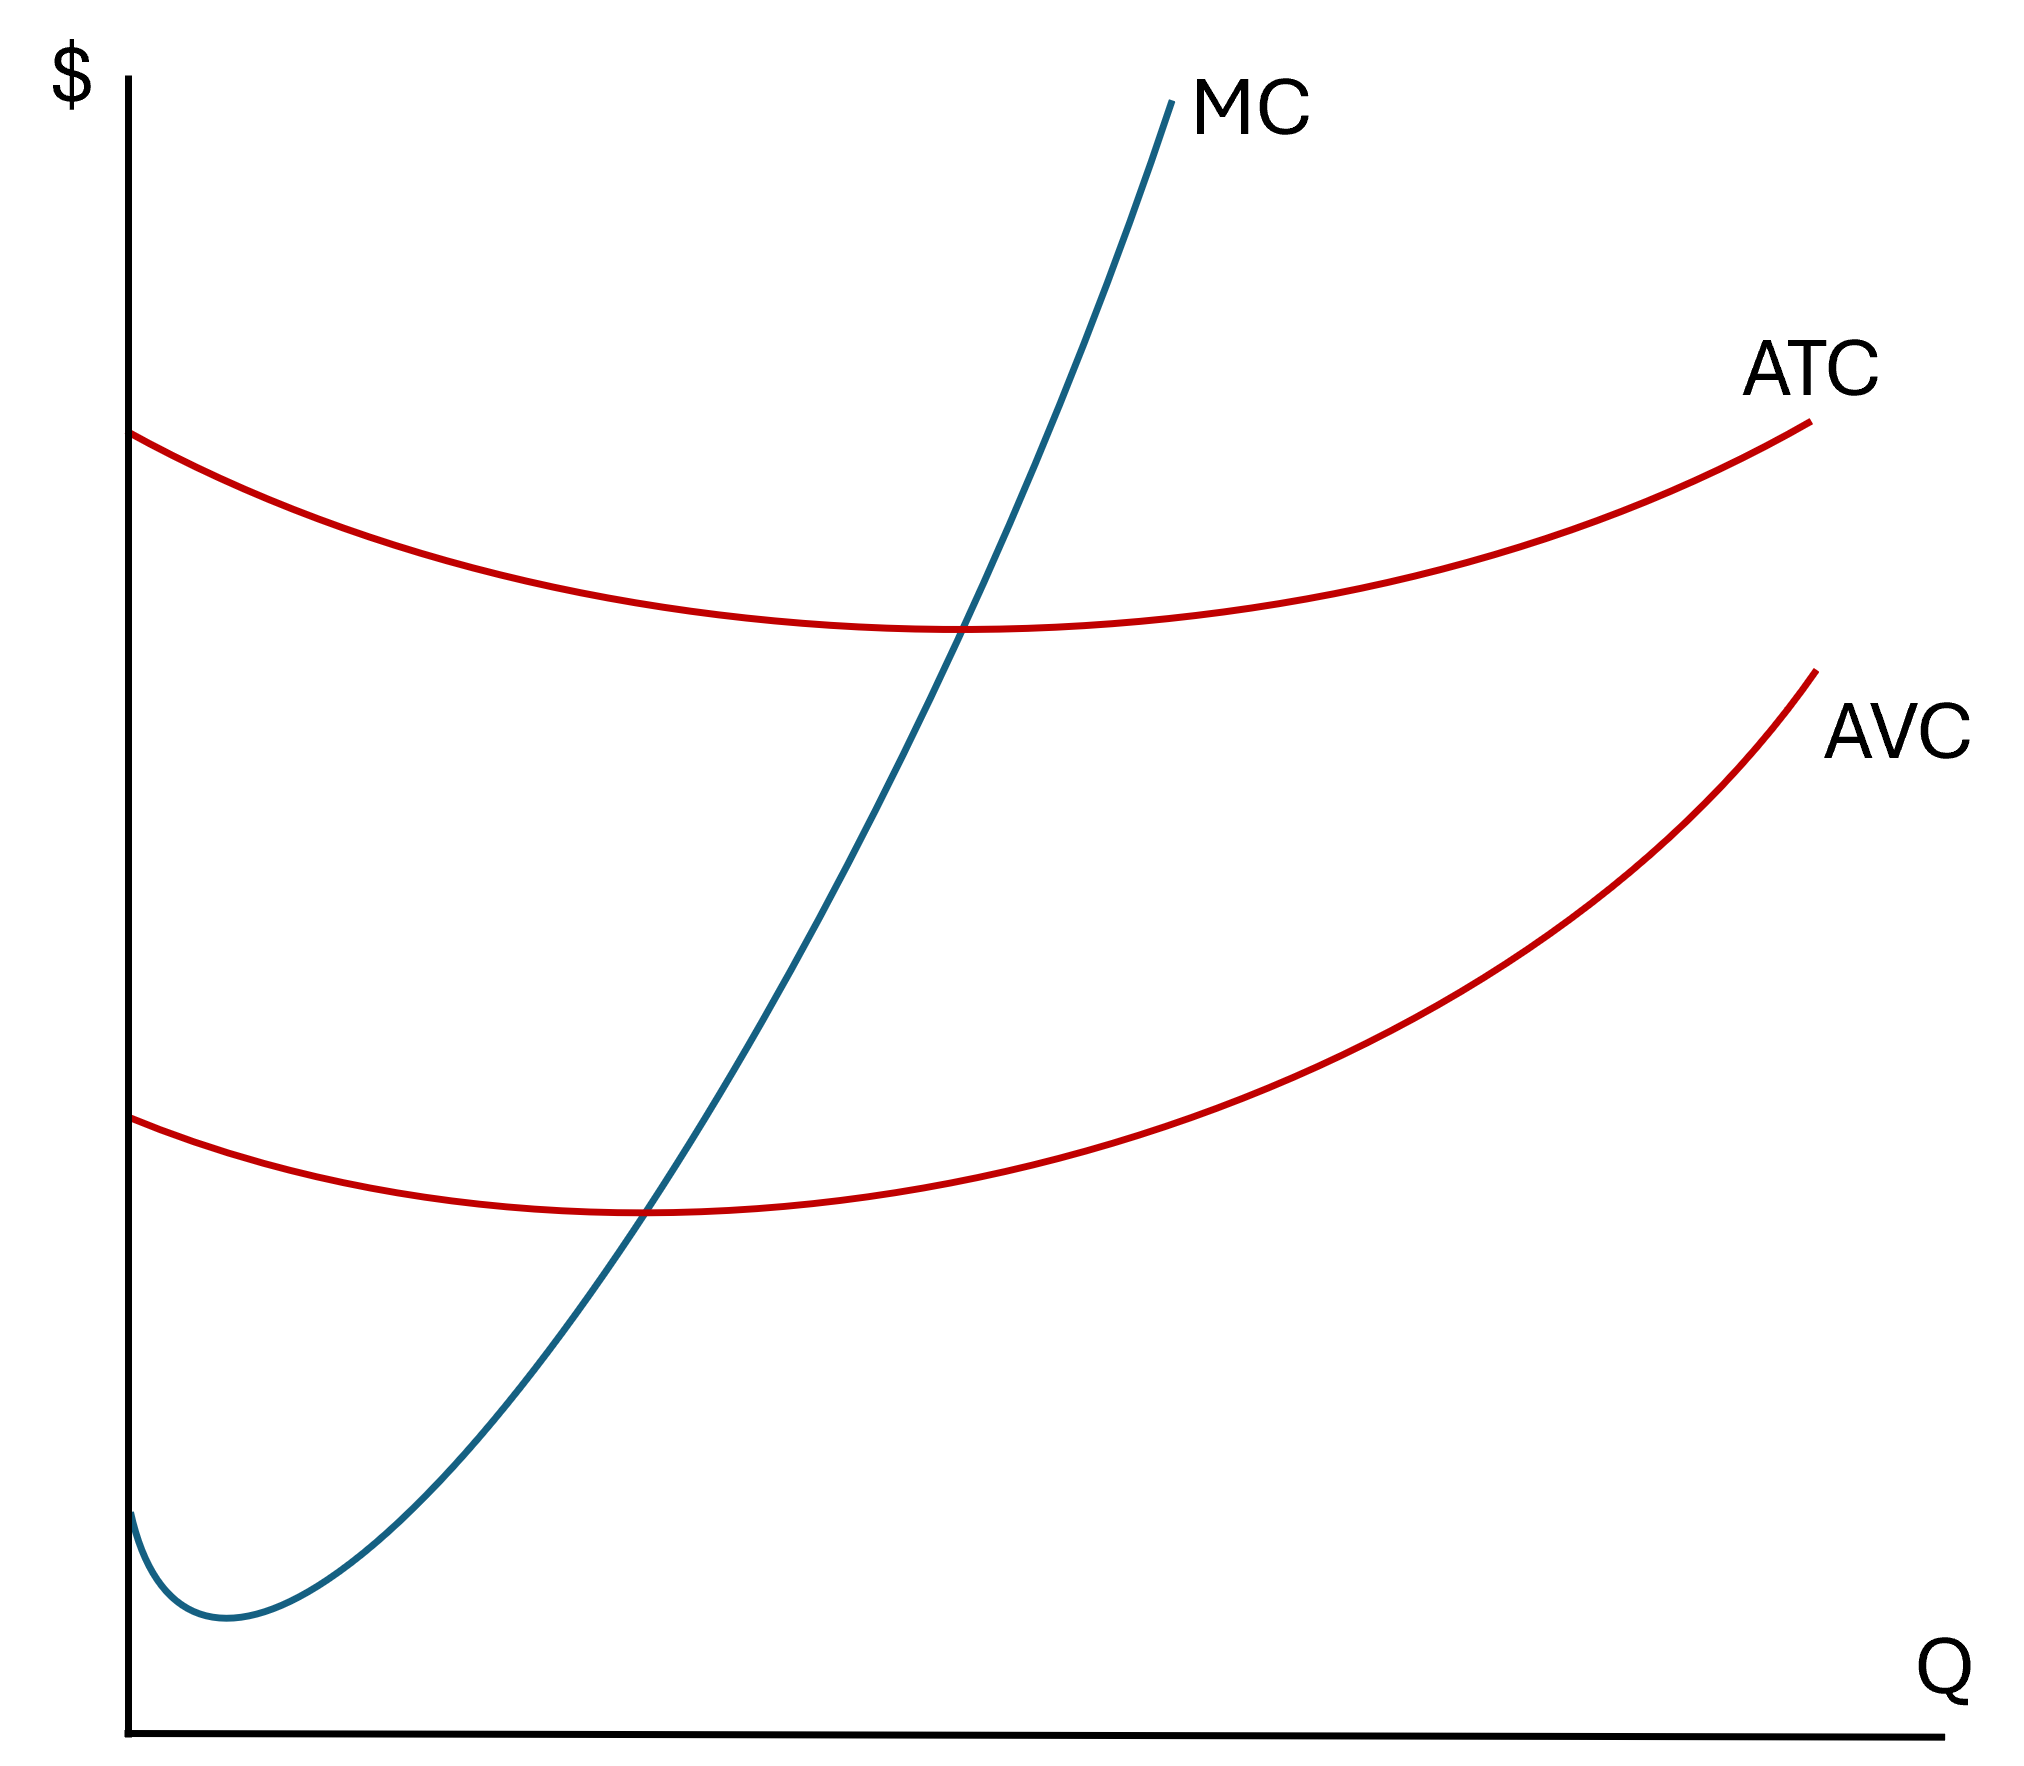
\includegraphics[width=\linewidth]{ATC.png}}
    \end{column}
\end{columns}
\end{frame}

\begin{frame}{Profit Maximization}
    \begin{columns}[c]
    \begin{column}{0.5\textwidth}
    Suppose the market is perfectly competitive, and the equilibrium price is $P$.\\
    \vspace{5pt}
    Which quantity should the firm produce?
    \vspace{5pt}
        \begin{itemize}
            \item<2-> Choosing $Q_1$ leaves money on the table: could produce more and still make positive marginal profits.
            \vspace{5pt}
            \item<2-> Choosing $Q_3$ makes negative marginal profits on the final units.
            \vspace{5pt}
            \item<2-> At $Q_2$ no improvement can be made. 
            \vspace{10pt}
            \item<2-> \textbf{Firms maximize profit by setting\\
            MR = MC.}
        \end{itemize}
    \end{column}
    \begin{column}{0.5\textwidth}
        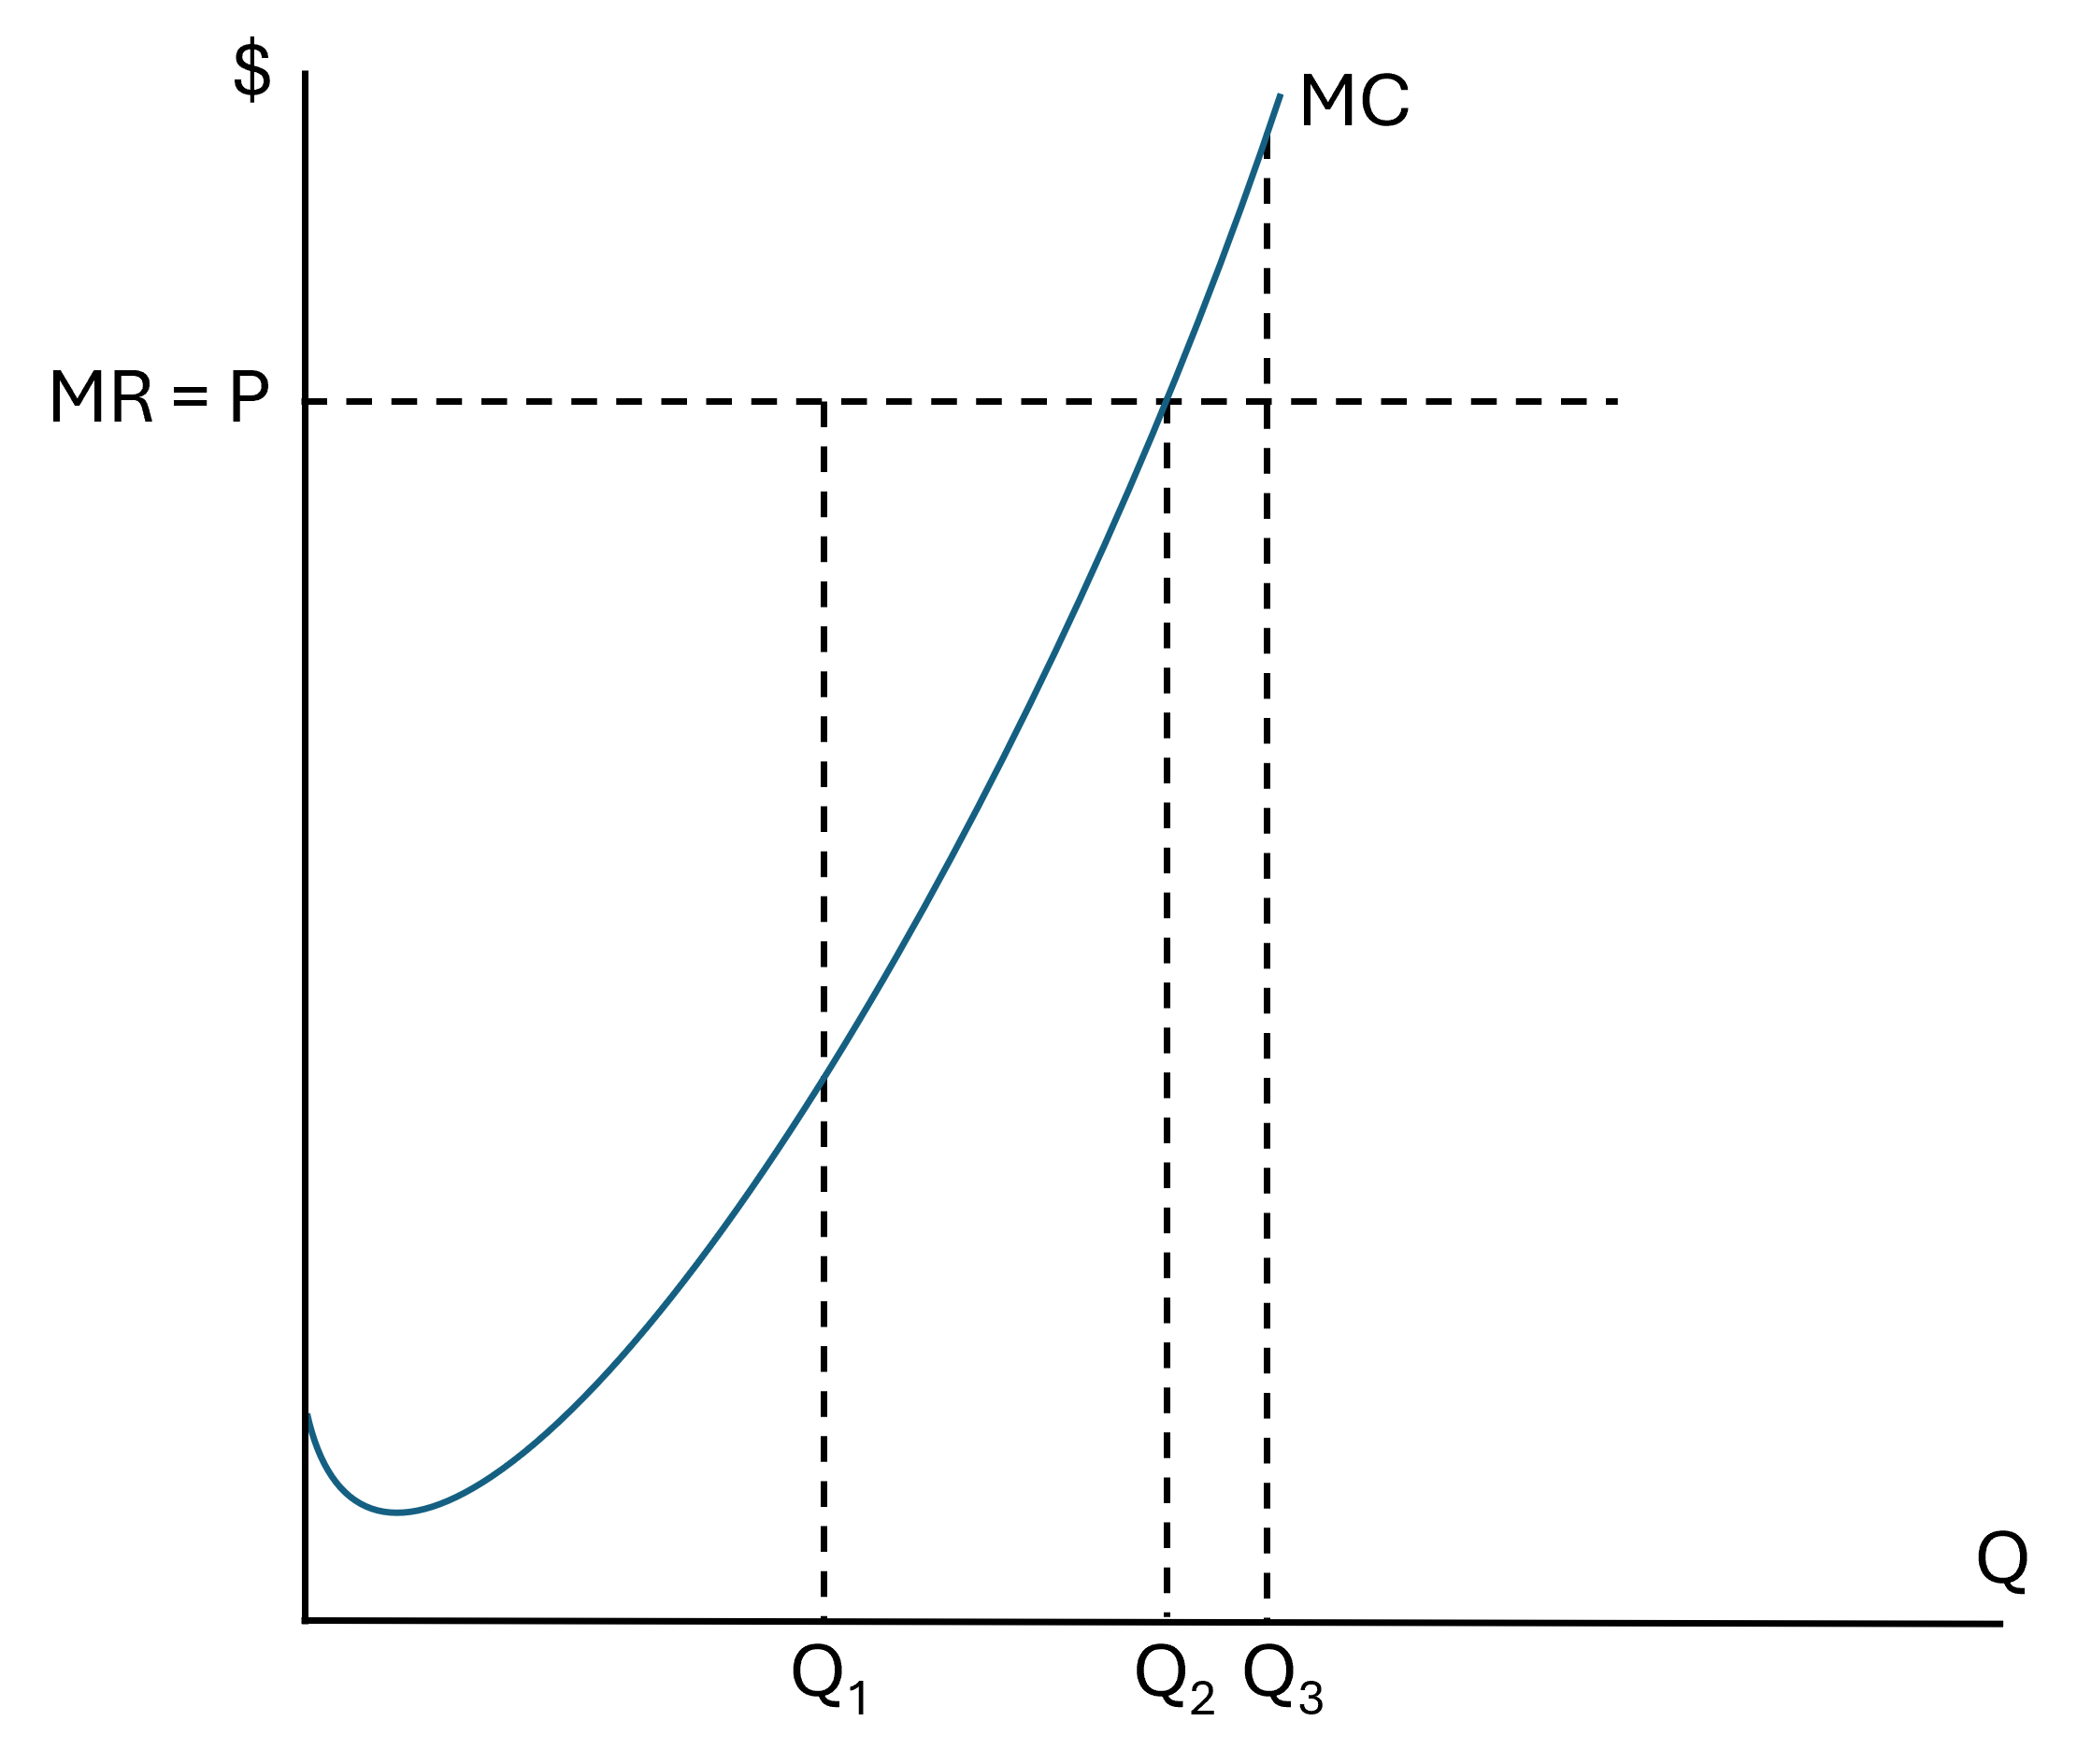
\includegraphics[width=\linewidth]{MC_again.png}
    \end{column}
\end{columns}
\end{frame}

\begin{frame}{Exercise 2: Cost Calculation}
    \begin{columns}[c]
        \begin{column}{0.5\textwidth}
        Given competitive market price $P$ and the pictured cost curves, calculate
        \vspace{5pt}
            \begin{enumerate}
                \item Total Revenue
                \item Total Cost
                \item Variable Cost
                \item Fixed Cost
                \item Profit
            \end{enumerate}
            \vspace{5pt}
            \textit{Hint}: \[TC = VC + FC\] \[AFC = FC/Q\] \[AVC = VC/Q\] \[ATC = TC/Q\]
        \end{column}
        \begin{column}{0.5\textwidth}
            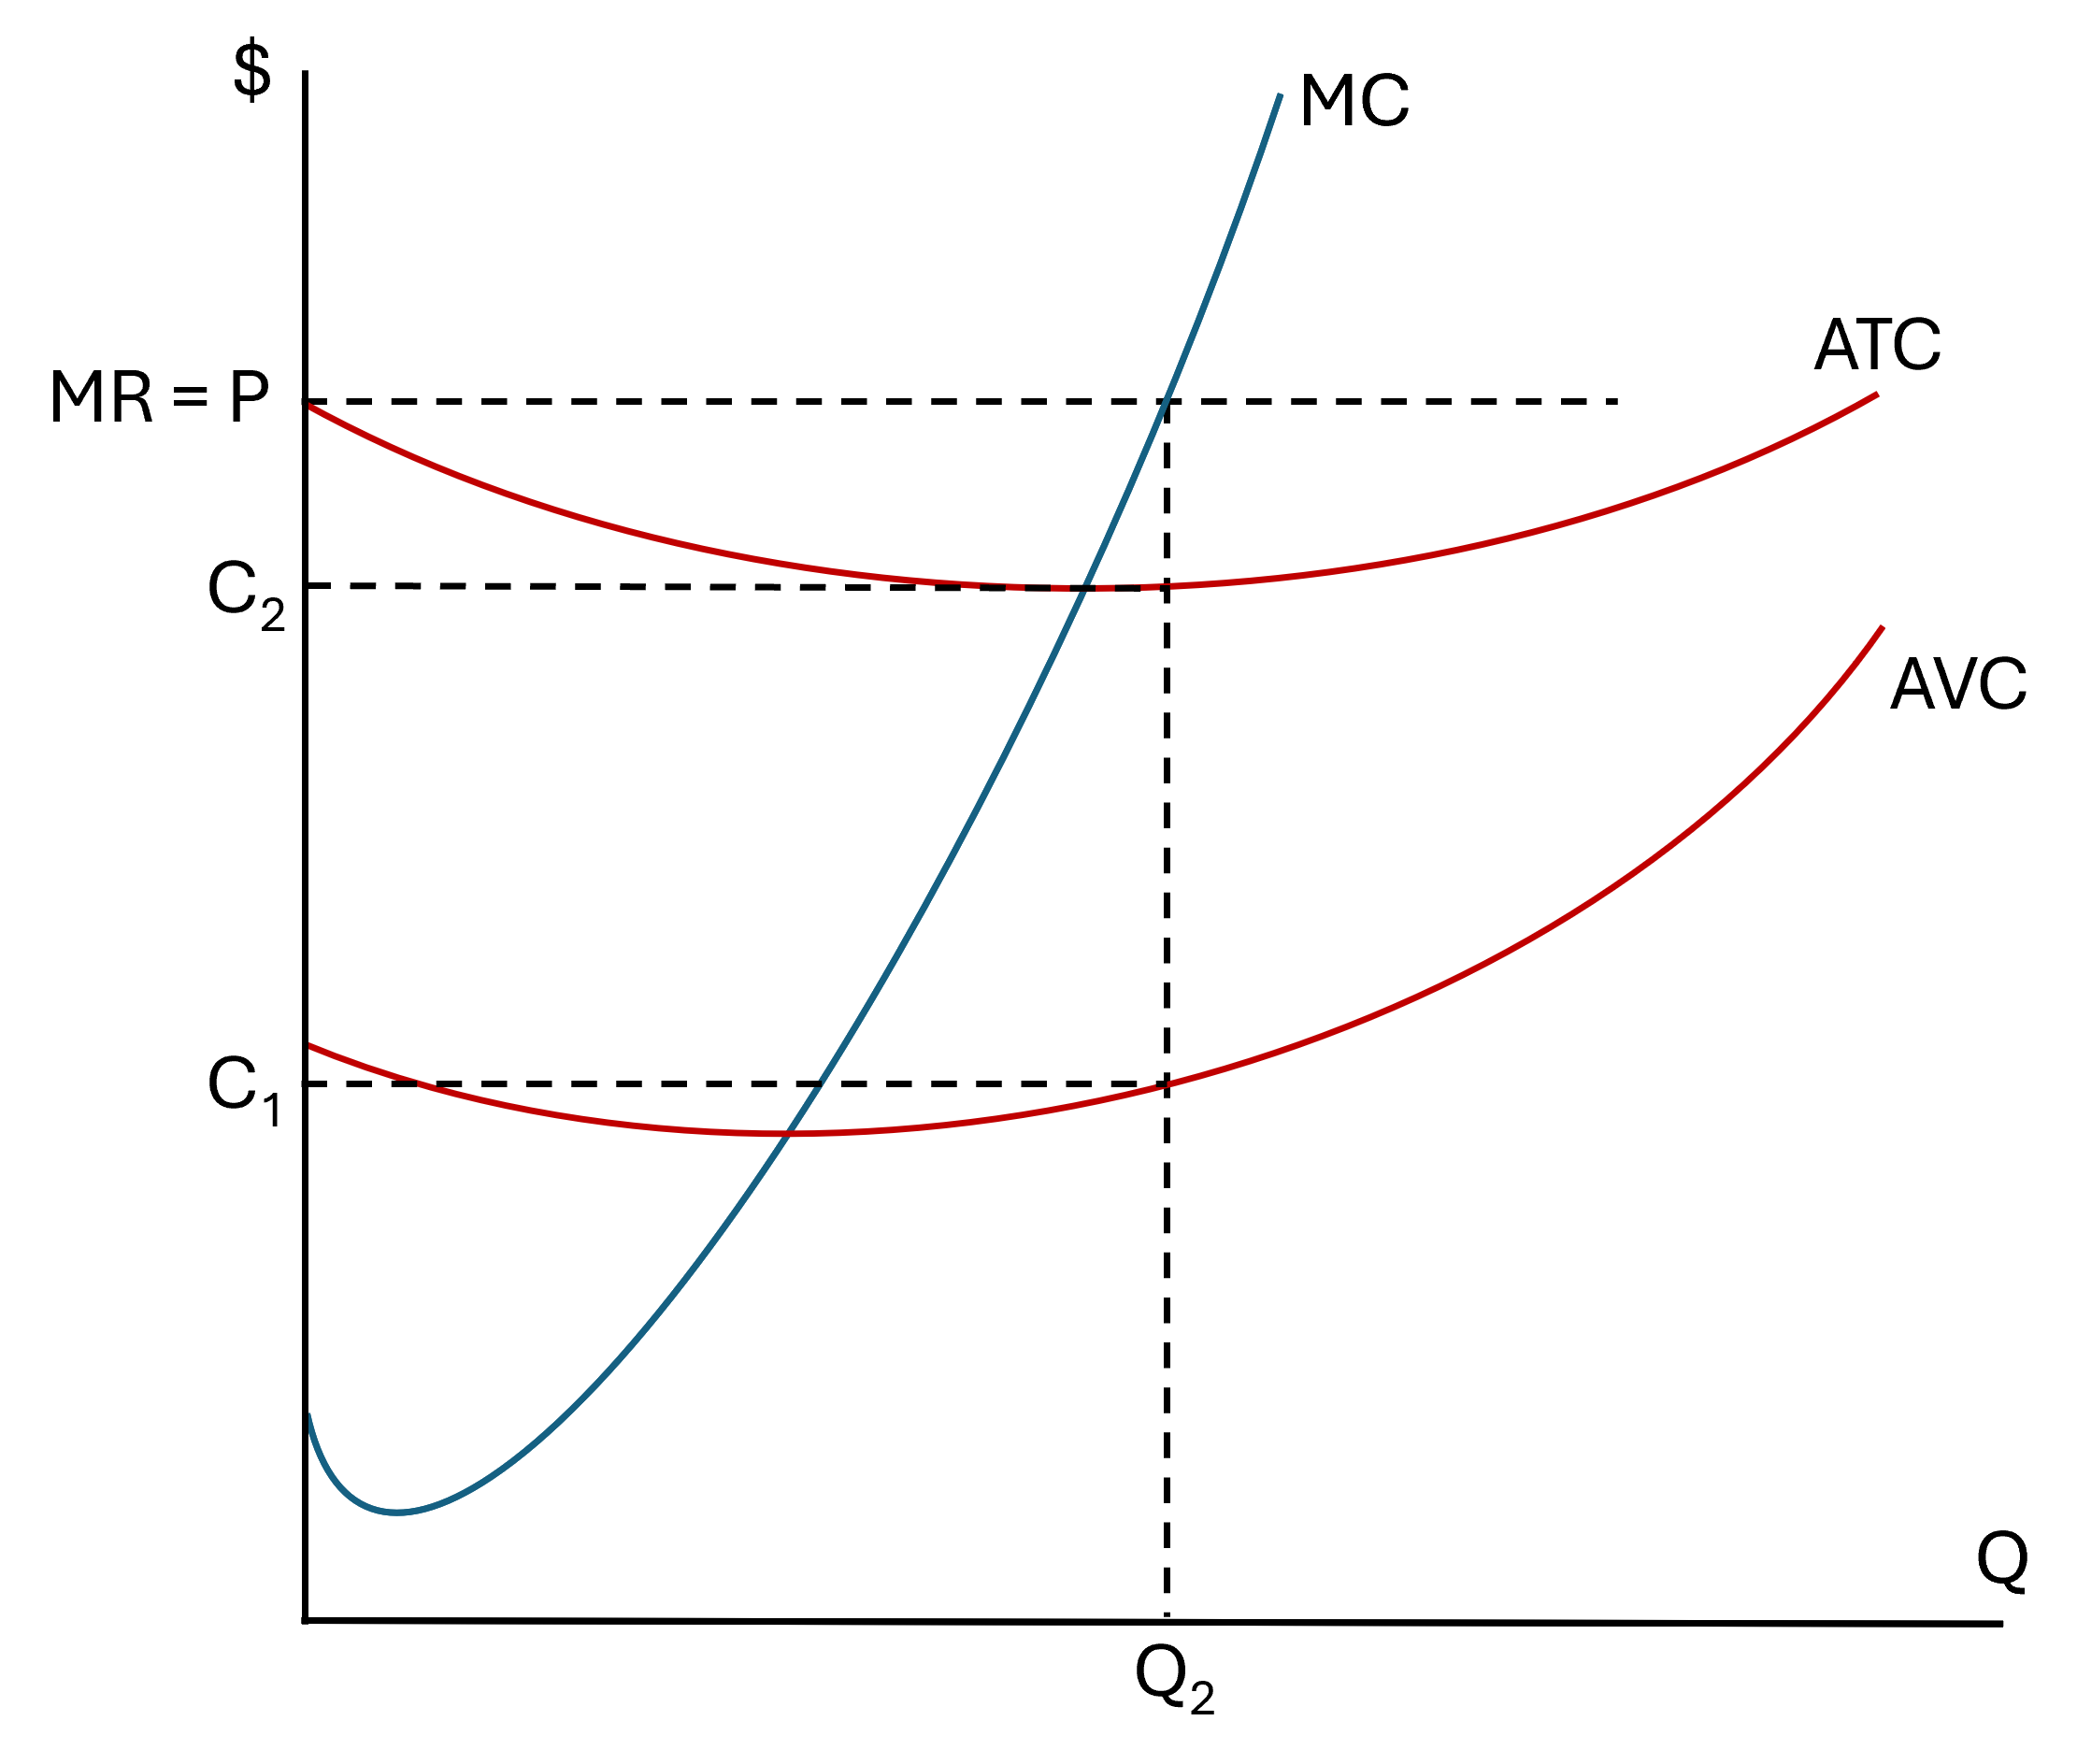
\includegraphics[width=\linewidth]{cost_exercise.png}
        \end{column}
    \end{columns}
\end{frame}

\begin{frame}{Exercise 2: Cost Calculation}
    \begin{columns}[c]
        \begin{column}{0.5\textwidth}
        Solution:\\
        \vspace{10pt}
        The firm maximizes profit by producing $Q_2$, where $MR = MC$.
        \vspace{5pt}
            \begin{enumerate}
                \item $TR = P \times Q_2$
                \item $TC = C_2 \times Q_2$
                \item $VC = C_1 \times Q_2$
                \item $FC = TC - VC = (C_2 - C_1) \times Q_2$
                \item $\Pi = TR - TC = (P - C_2) \times Q_2$
            \end{enumerate}
        \end{column}
        \begin{column}{0.5\textwidth}
            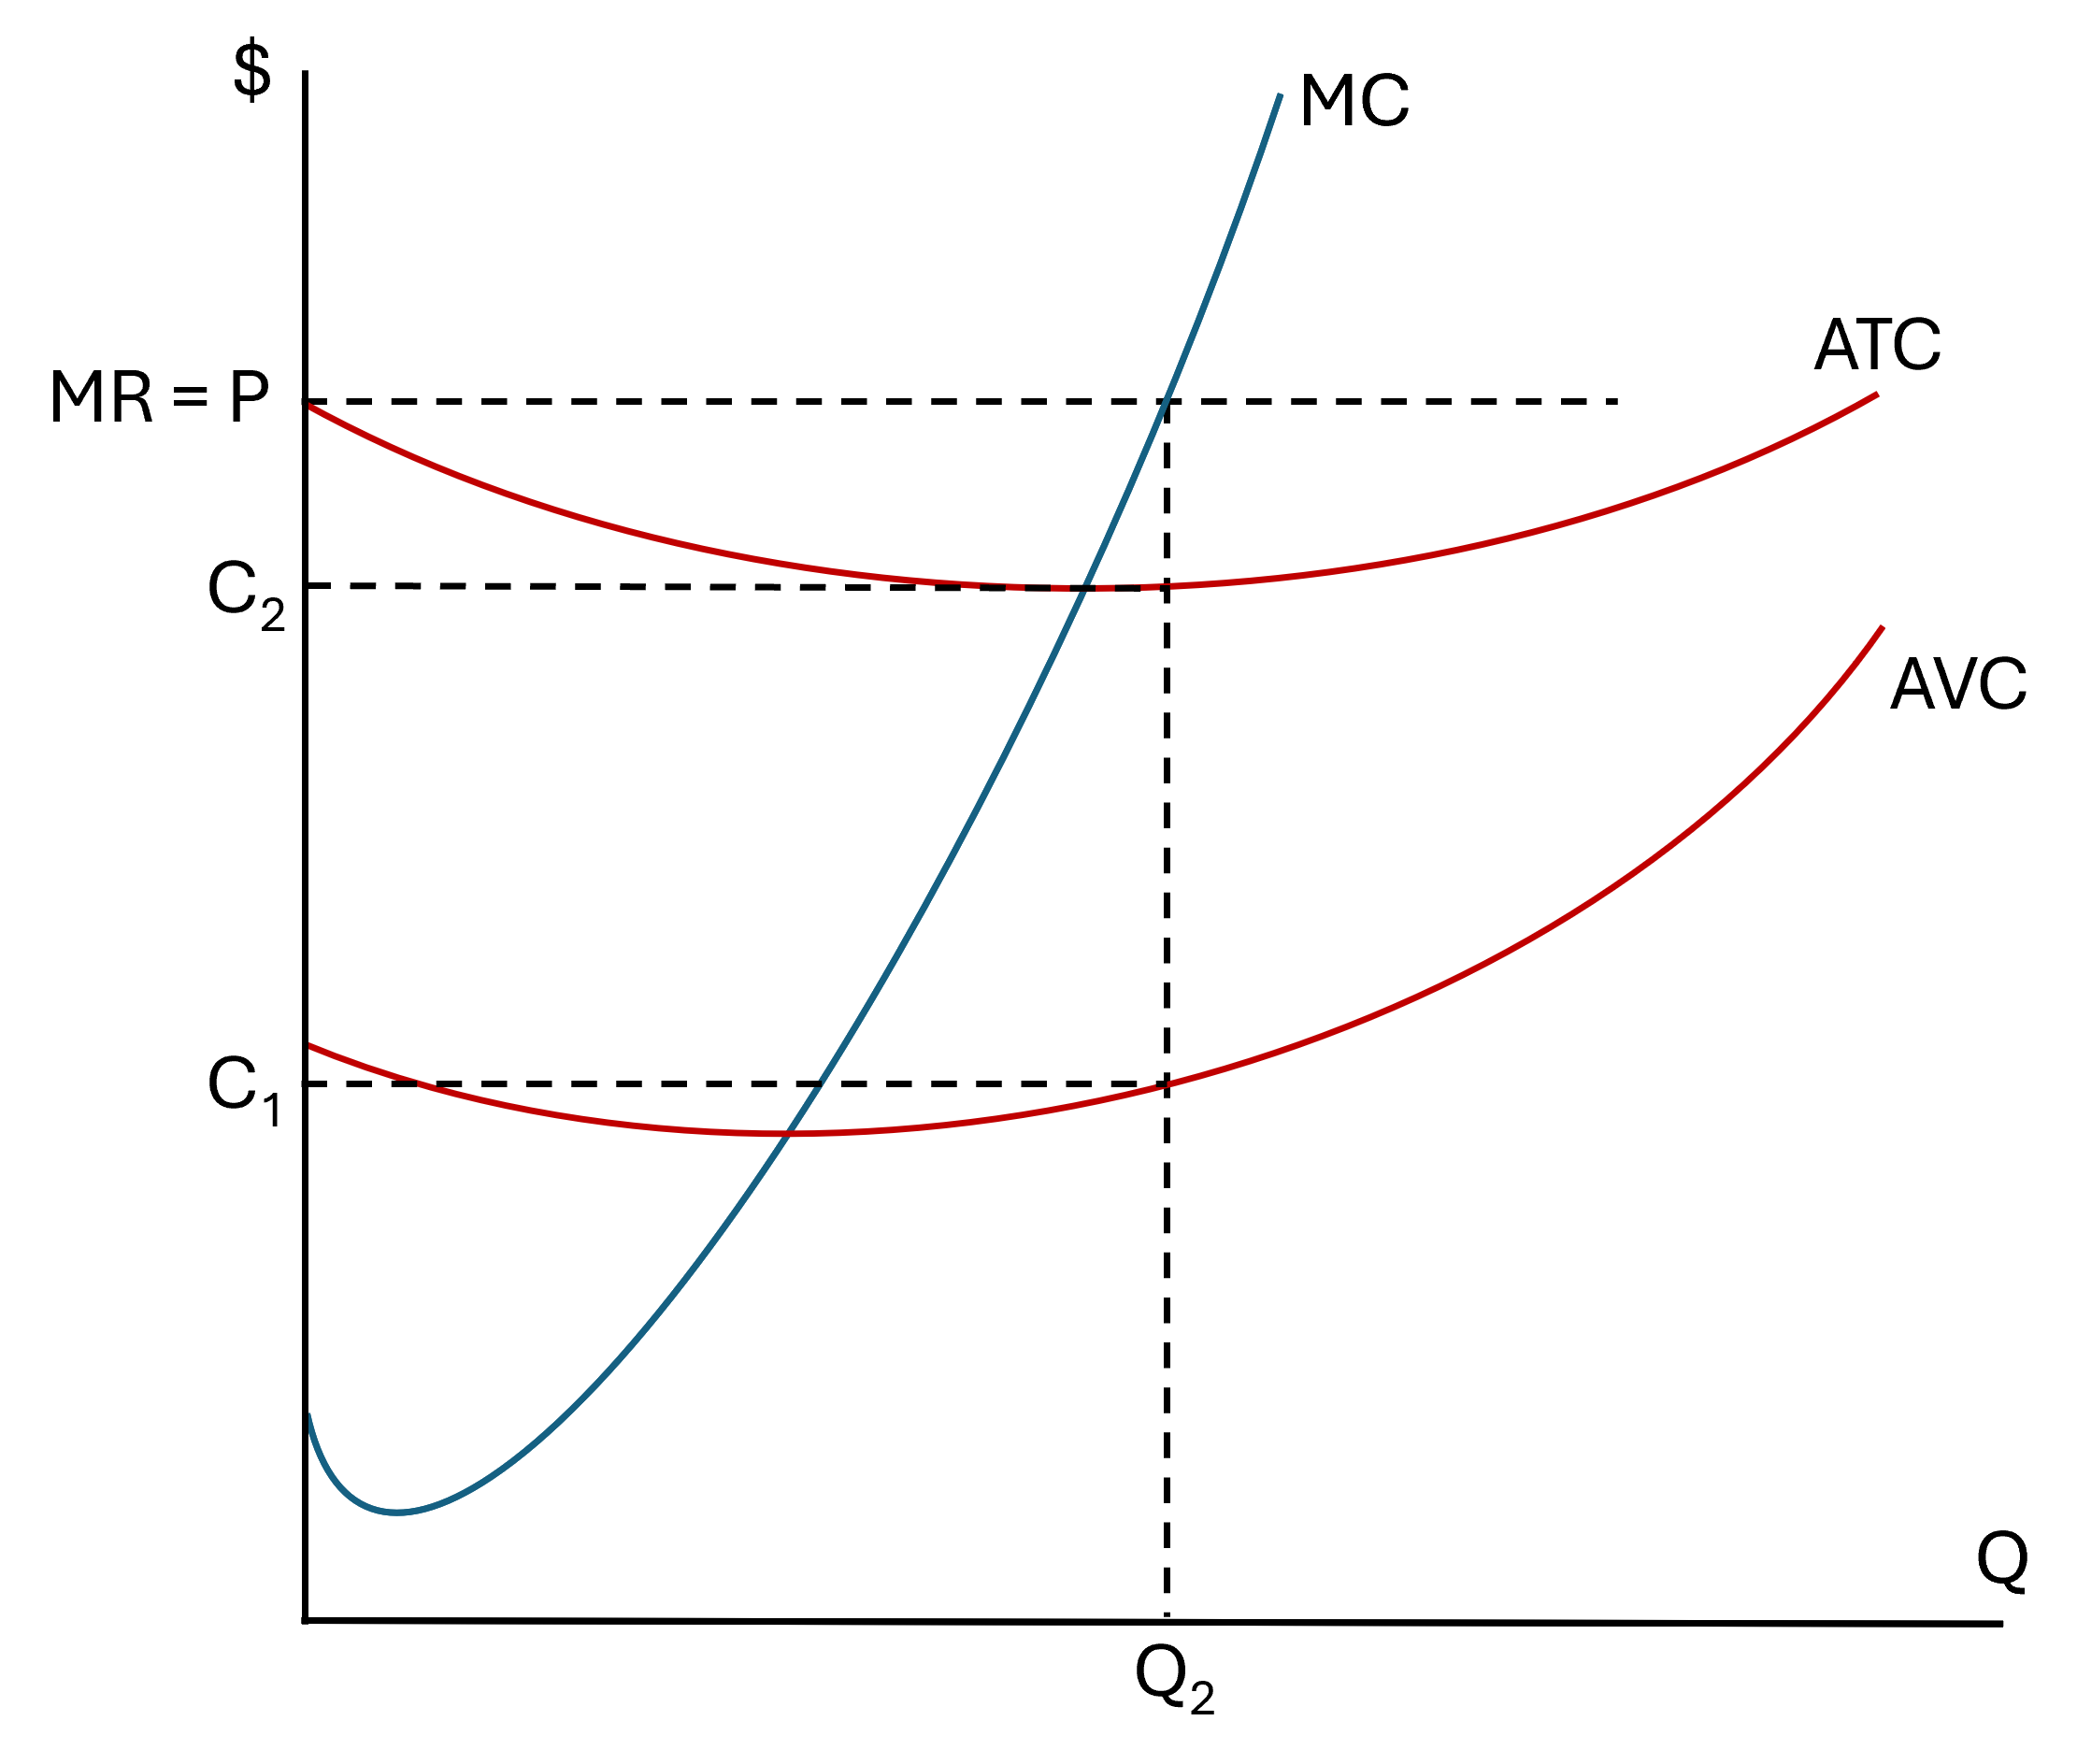
\includegraphics[width=\linewidth]{cost_exercise.png}
        \end{column}
    \end{columns}
\end{frame}

\begin{frame}{The Supply Curve}
    \begin{columns}[c]
    \begin{column}{0.5\textwidth}
        \begin{itemize}
            \item<1-> \textbf{Firms maximize profit by setting\\
            MR = MC.}
            \item[$\rightarrow$]<1->  The marginal cost curve describes the relationship between price and quantity supplied.
            \vspace{10pt}
            \item<2-> For a competitive market (where $P = MR$), the MC curve \textit{is the firm's supply curve!}
        \end{itemize}
    \end{column}
    \begin{column}{0.5\textwidth}
        \only<1>{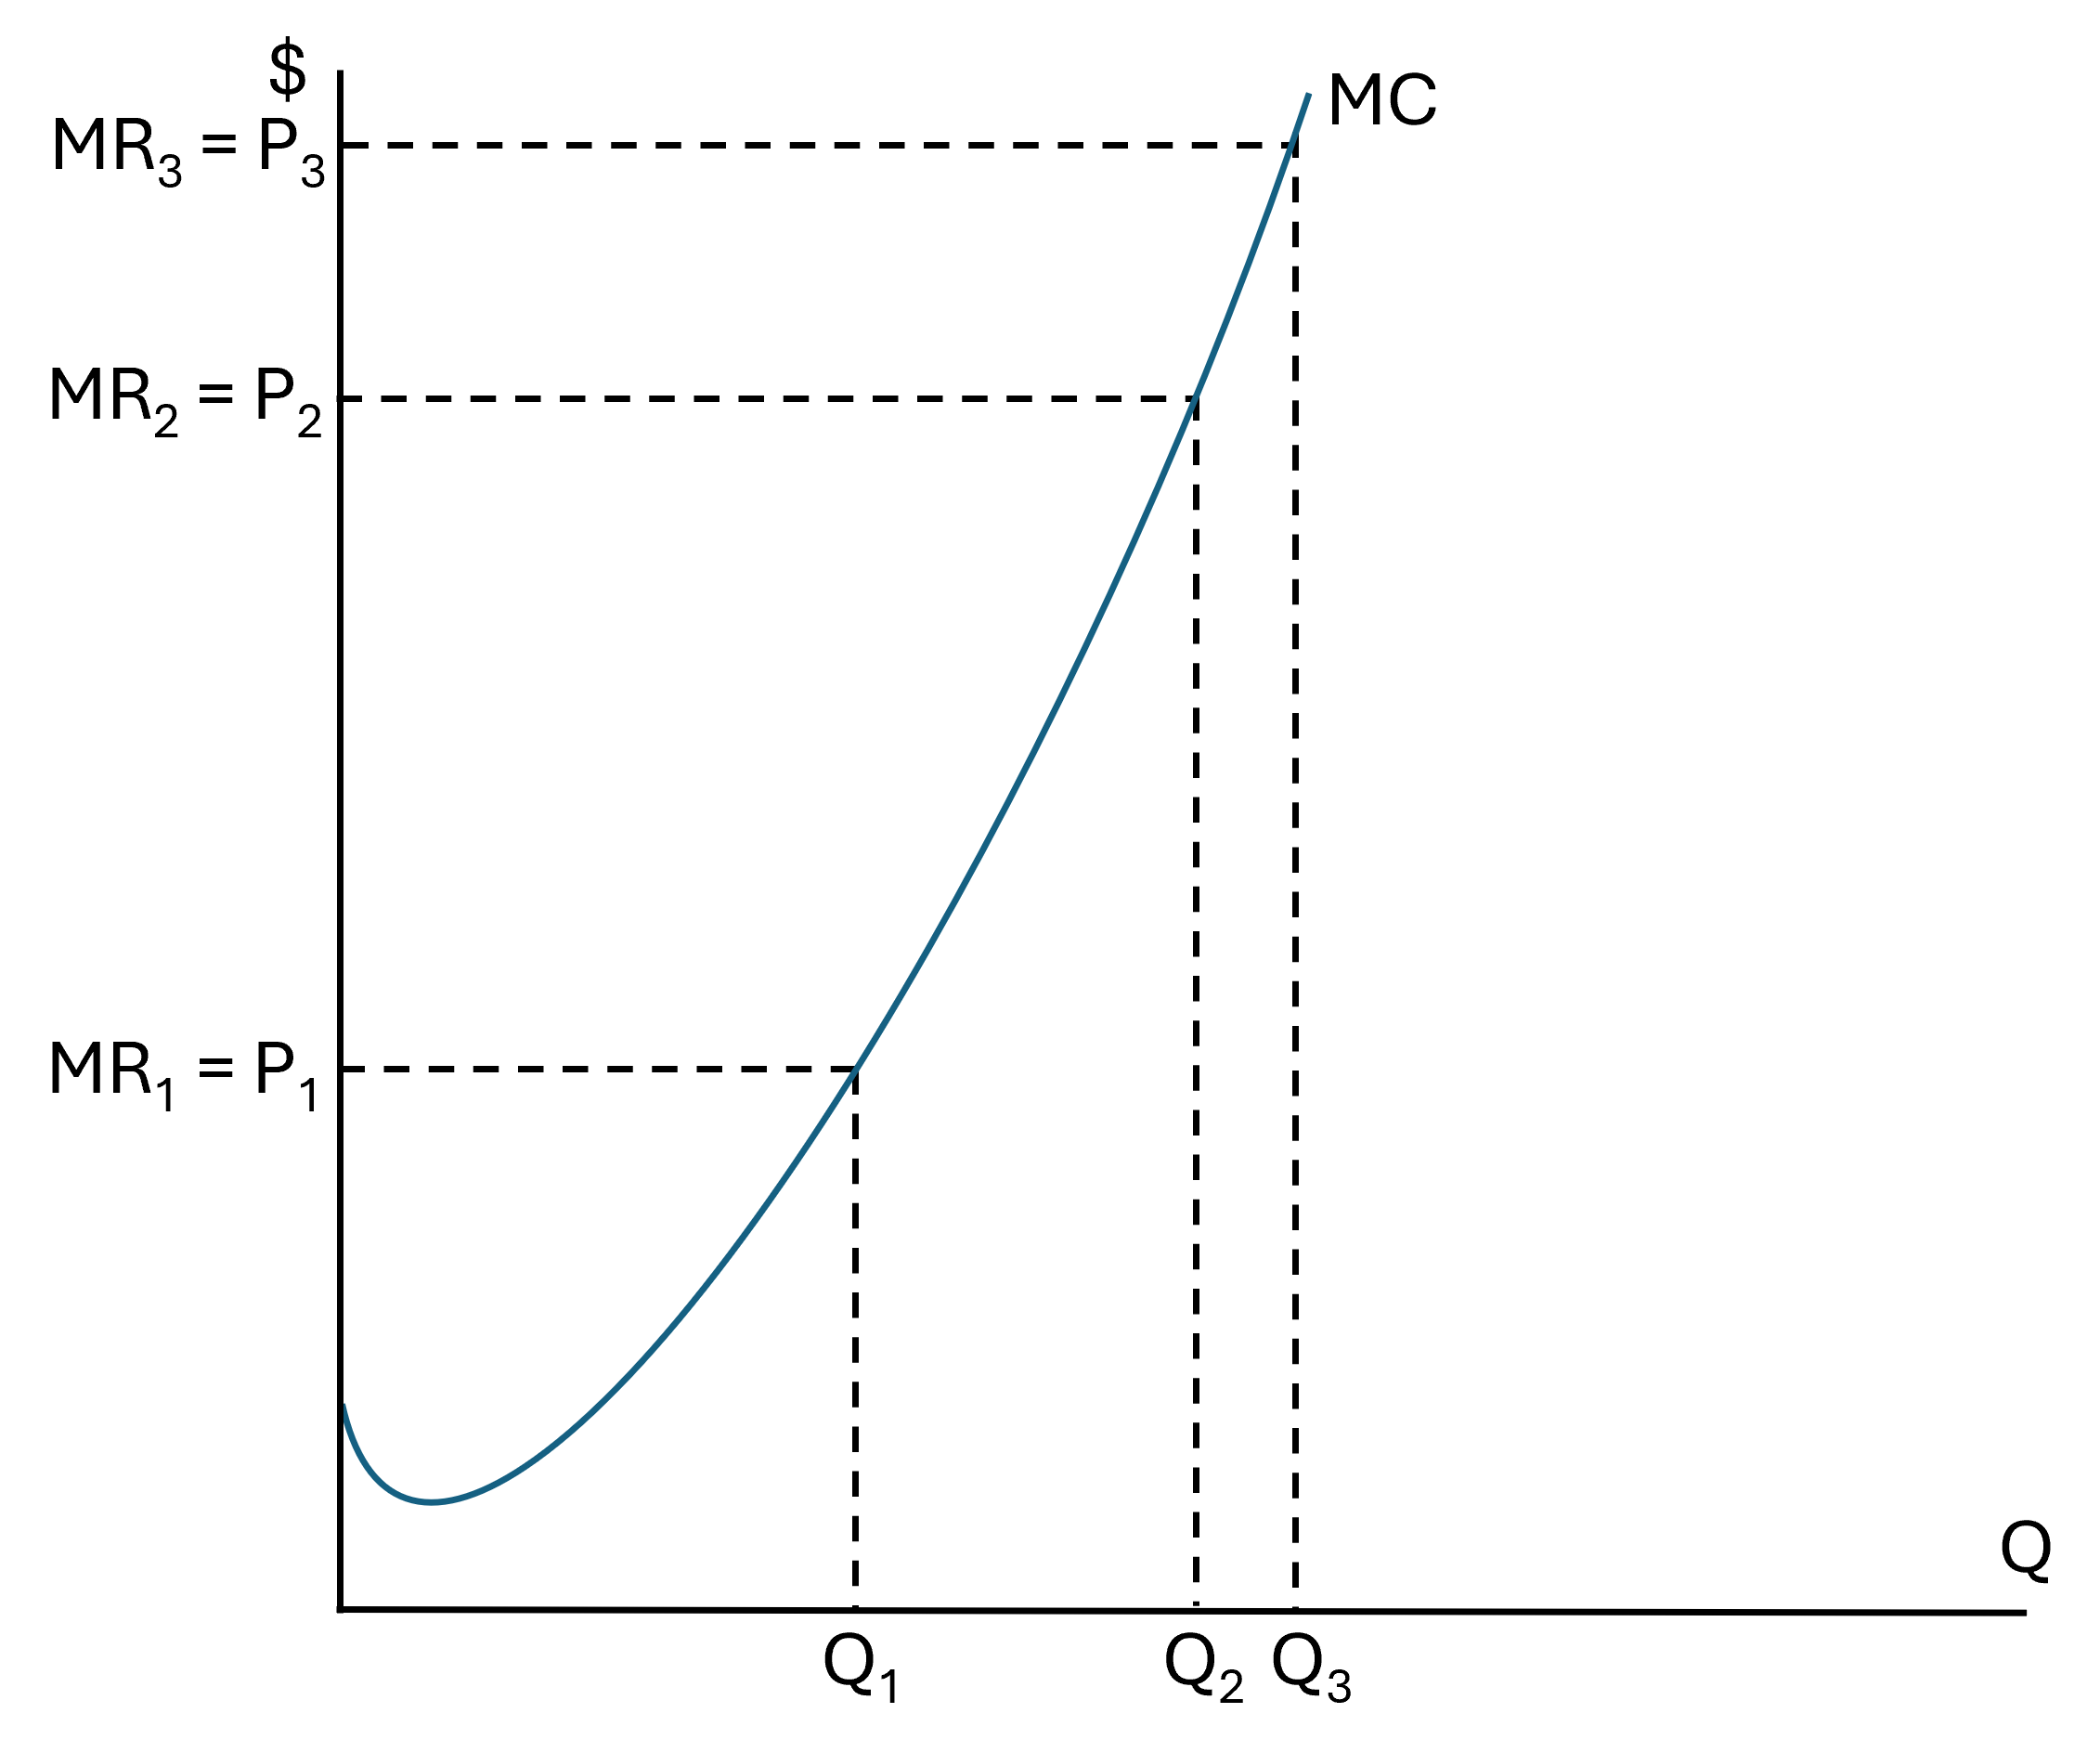
\includegraphics[width=\linewidth]{MC_price.png}}
        \only<2>{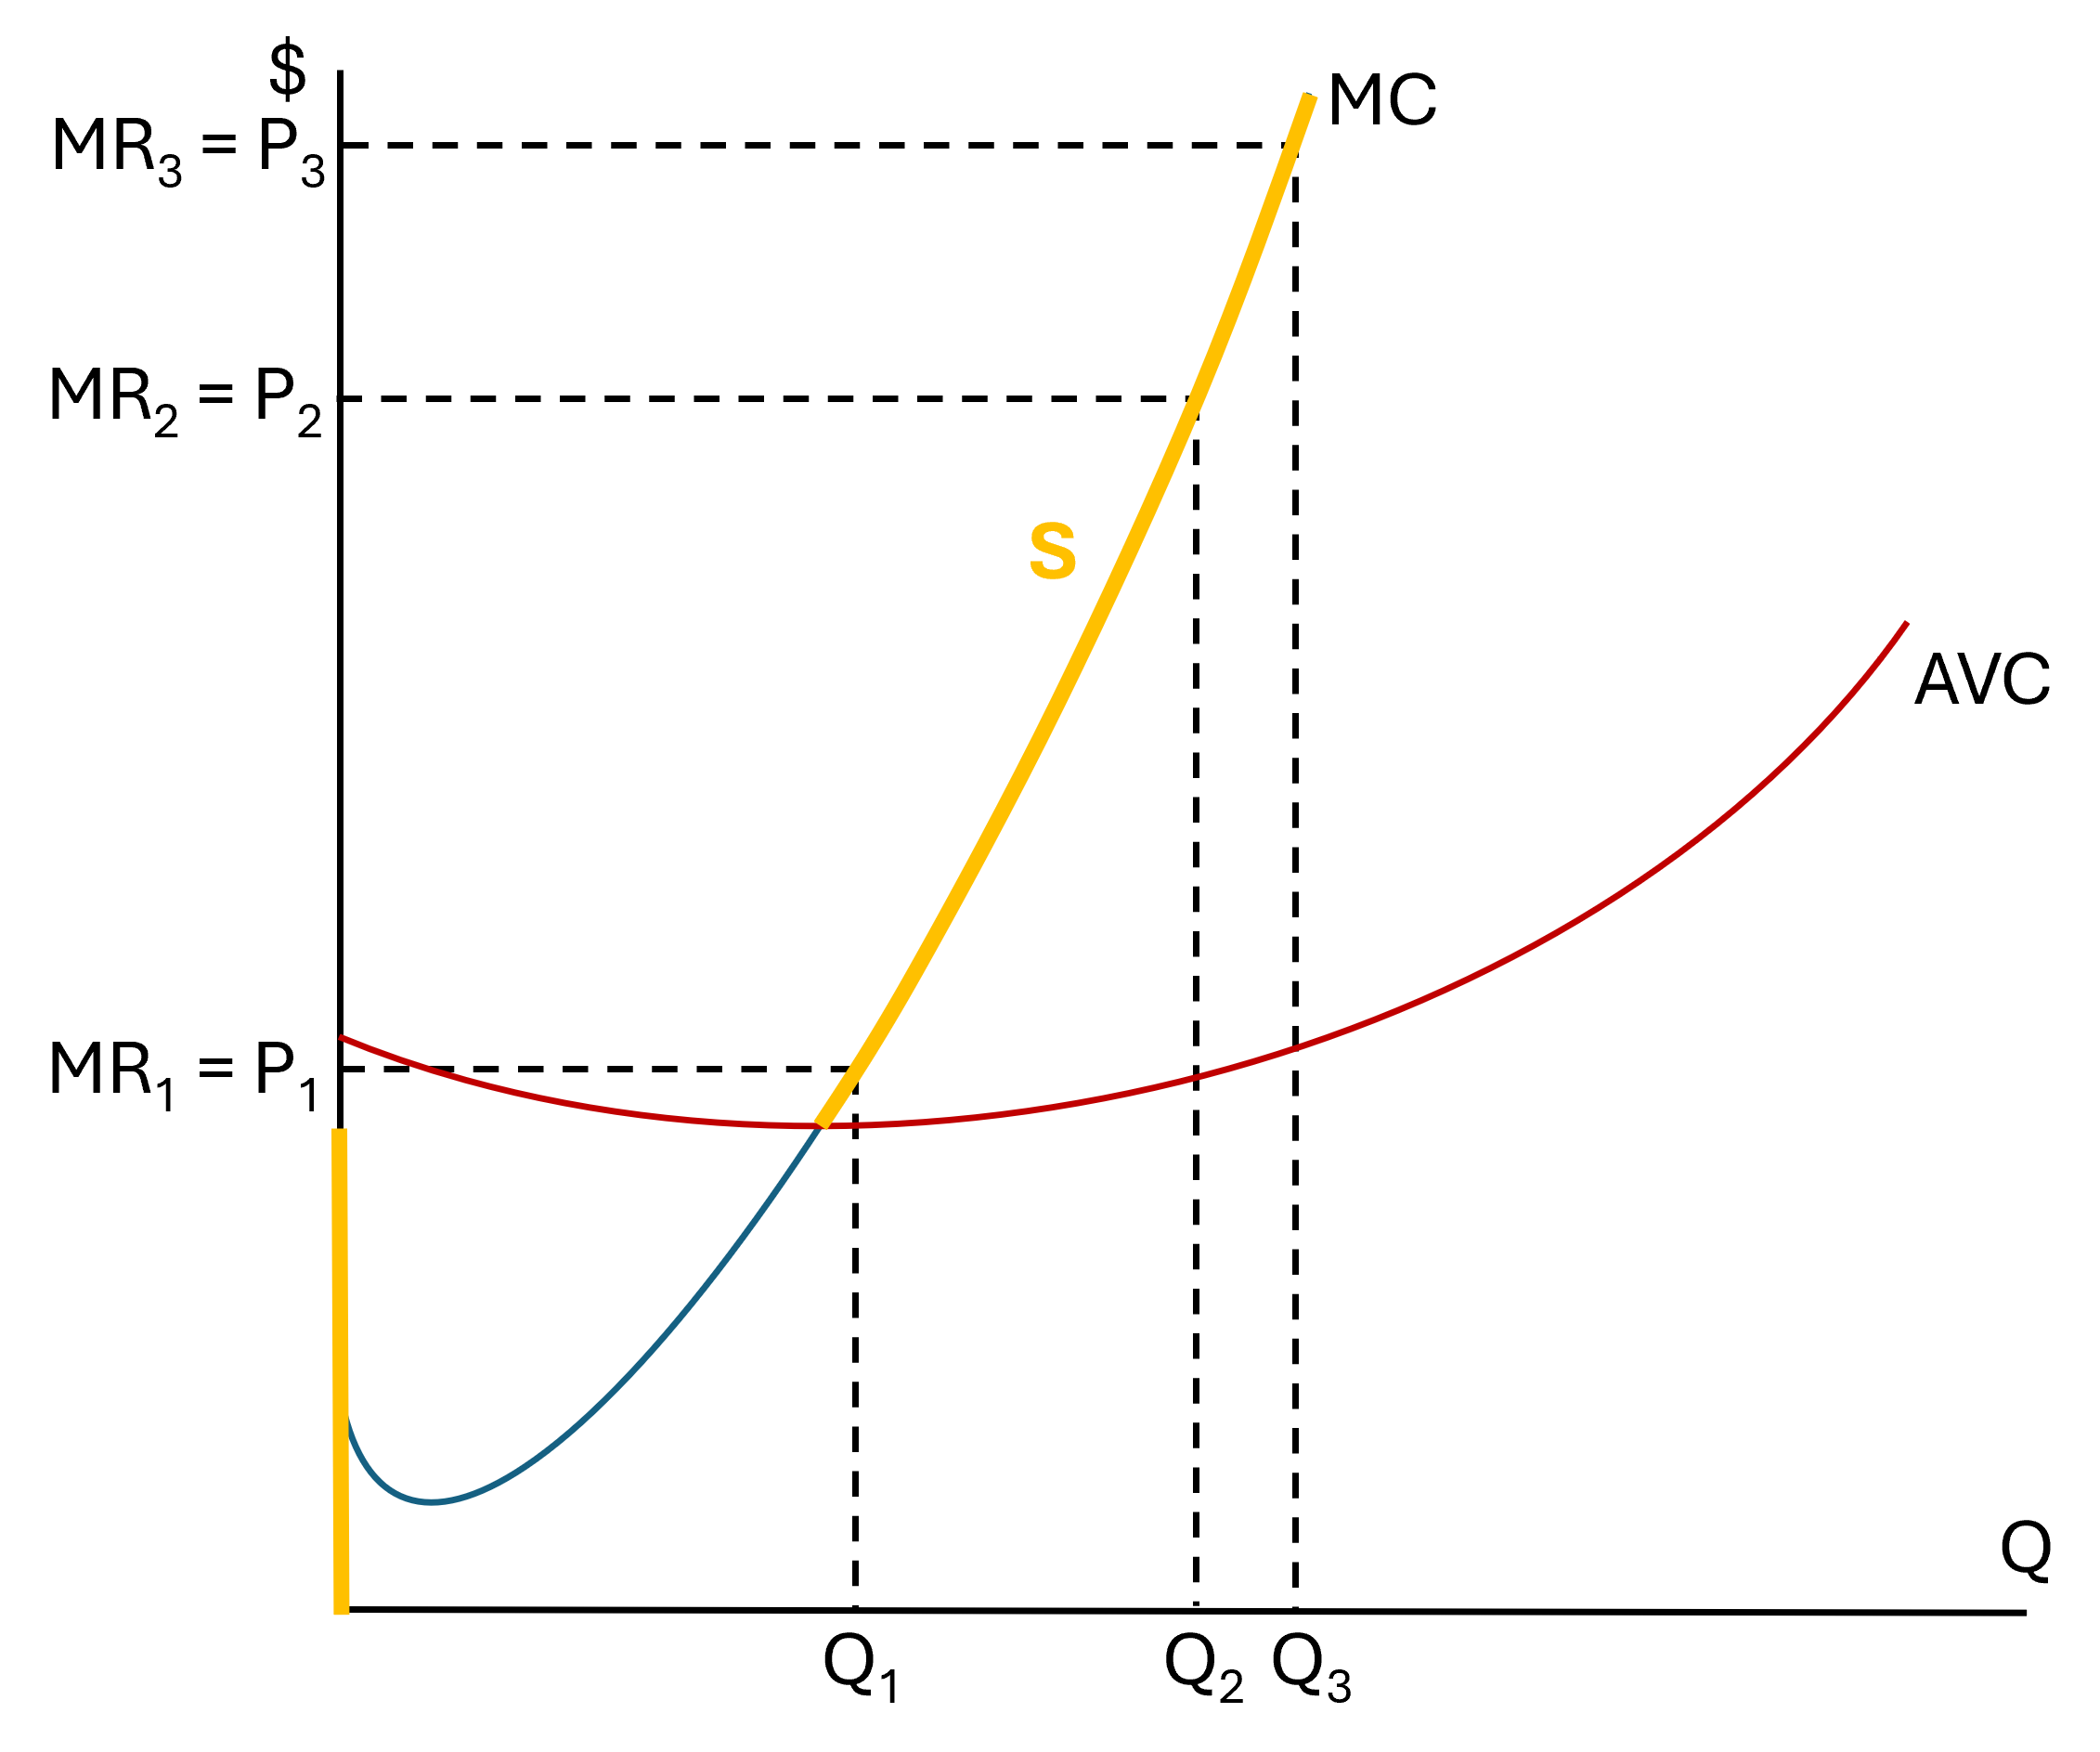
\includegraphics[width=\linewidth]{supply.png}}
    \end{column}
\end{columns}
\end{frame}

% \begin{frame}{Exercise 2: Cost Curves}
%     The following graph plots the cost curves of Jane's Juice Bar. \\
%     Q1: What is the relationship between MC, AVC, and ATC? Why?
%     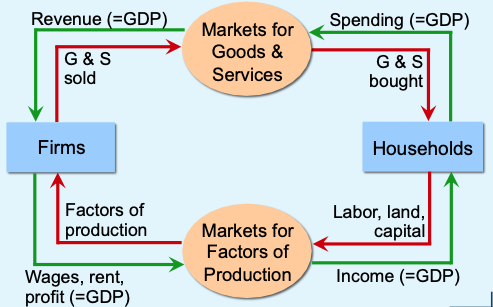
\includegraphics[scale=0.4]{fig1.png}
% \end{frame}

% \begin{frame}{Exercise 2: Cost Curves}
%     Solution: \\
%     MC intersects with AVC at the lowest point of AVC. Same for ATC. 
% \end{frame}

\end{document}
